\section{Metodología}

El diagrama \ref{fig:metodologia} muestra el flujo de la metodología realizada para el proyecto. Esta forma de trabajo está inspirada en la forma en la que se estructuran en su gran mayoría los proyectos de aprendizaje automático, sin tener en cuenta re-entrenamiento u otros aspectos de tener un modelo en productivo a lo largo del tiempo.

\begin{figure}
    \centering
    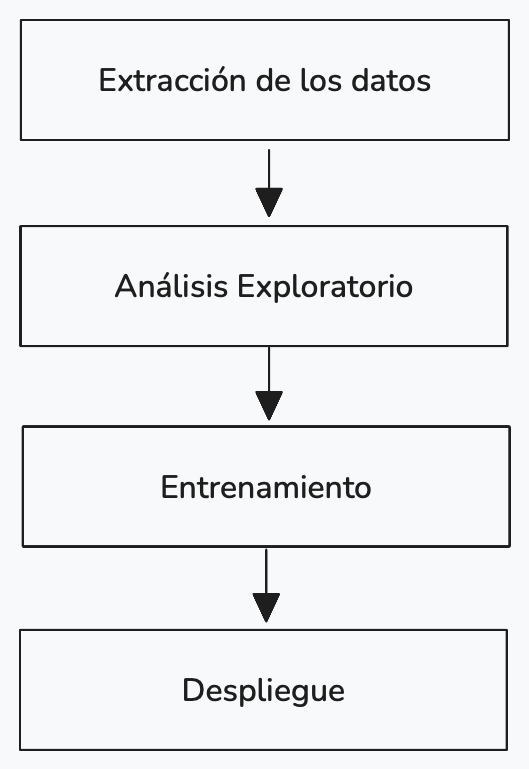
\includegraphics[width=0.2\textwidth]{resources/metodologia.png}
    \caption{Diagrama de la metodología utilizada}
    \label{fig:metodologia}
\end{figure}


\subsection{Extracción de los datos}

En primer lugar, la extracción de los datos tuvo dos momentos principales. En primer lugar, se intentó realizar una extracción manual de los datos, utilizando el \verb|API| público de reddit y el wrapper \verb|PRAW|. Sin embargo este proceso resultó costoso en términos de tiempo y recursos computacionales, y por restricciones del dominio no se podían conseguir más de 2000 publicaciones en un solo llamado. Todos estos procesos e intentos se encuentran documentados en el repositorio.

El hecho de tener un dataset pequeño no era problemático en sí, ya que se lograban extraer posts lo suficientemente largos. Sin embargo, el problema era el desbalance de clases, ya que, incluso en el nuevo dataset, conseguir clases que sean diferentes a YTA o NTA es demasiado difícil, ya que esos veredictos son muy poco comunes, por lo que en este primer intento a veces no se conseguían publicaciones de todas las clases.

Es por ello que se hizo una búsqueda de otro dataset, con el cual se llegó a una base de datos \verb|SQLite| \cite{liew2023reddit}. Este dataset  es mucho más grande de lo que podríamos haber obtenido manualmente, y probó ser un gran insumo para el proyecto. 

\subsection{Análisis Exploratorio}

Antes de proceder con la implementación y evaluación de modelos de lenguaje, se realizó un análisis exploratorio exhaustivo del conjunto de datos extraído del subreddit r/AmITheA**hole. Este análisis tuvo como propósito comprender la estructura del corpus, caracterizar la distribución de etiquetas morales y explorar el comportamiento de los usuarios frente a distintos tipos de publicaciones. Para ello, se procesaron datos provenientes de una base SQLite que almacenaba tanto las publicaciones originales como los comentarios emitidos por la comunidad, permitiendo así una inferencia automatizada de etiquetas de juicio moral.

\subsubsection*{Tamaño, distribución y metainformación}

El conjunto de datos procesado consta de \textbf{30.830 publicaciones} recopiladas entre octubre de 2022 y noviembre de 2023. A cada entrada se le asignó una etiqueta de juicio moral (\texttt{YTA}, \texttt{NTA}, \texttt{ESH}, \texttt{NAH}, \texttt{INFO}) mediante el conteo de menciones explícitas en los comentarios de los usuarios, considerando como \emph{gold label} aquella más frecuente. La distribución resultante refleja un claro desbalance de clases, con predominancia de la etiqueta \texttt{NTA} (81.4\%), seguida por \texttt{YTA} (17.3\%), mientras que las restantes categorías representan menos del 1\% cada una. 

\subsubsection*{Tendencias, información adicional} Además, se observó que las publicaciones con veredictos \texttt{YTA} no necesariamente tienden a generar mayor controversia. Esta información resulta clave para interpretar los retos de clasificación y los posibles sesgos en modelos de aprendizaje automático entrenados sobre estos datos, ya que vemos que no hay correlaciones entre estas métricas de las publicaciones. A continuación se muestran algunas de las distribuciones sobre los datos que son particularmente interesantes. Estas tendencias se visualizan con la figura \ref{fig:tendencias}.\footnote{El análisis completo con todas las distribuciones se encuentra en el cuaderno de Jupyter correspondiente, el cual se puede consultar en el repositorio (ver sección \ref{sec:experimentos}).} 

\begin{figure}
    \centering
    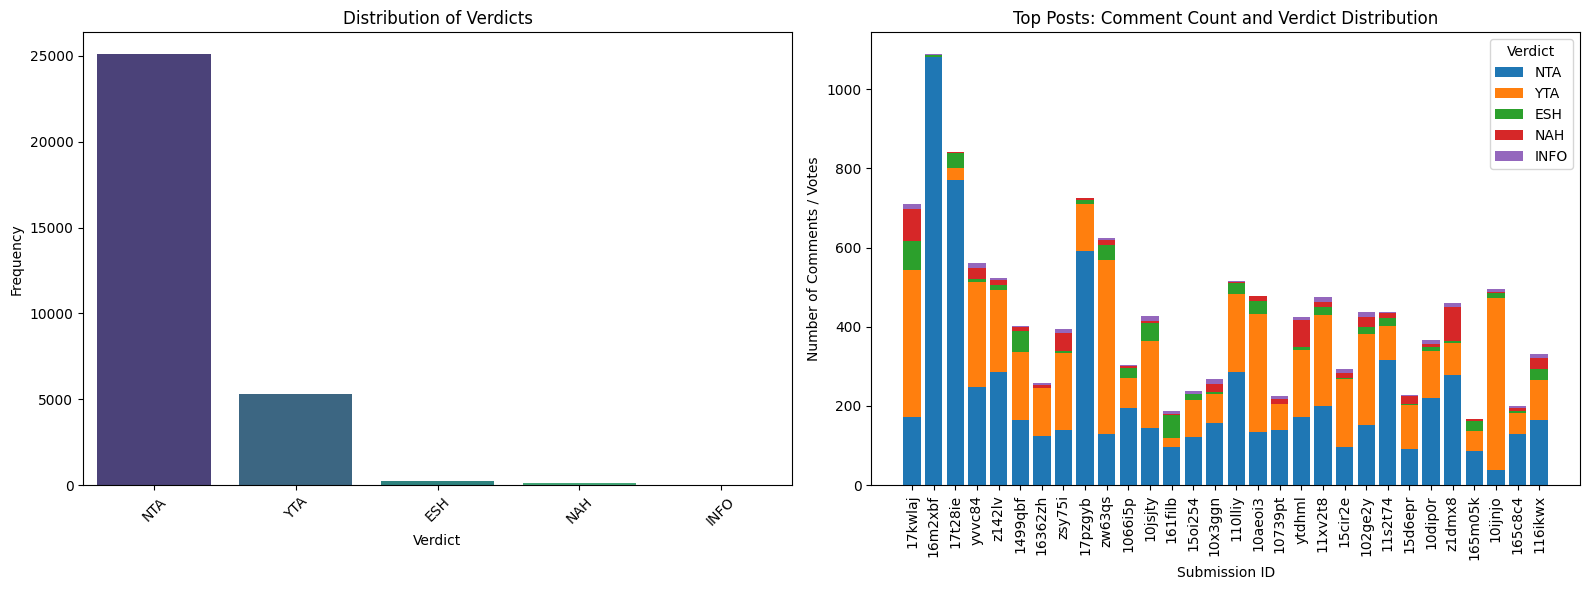
\includegraphics[width=0.45\textwidth]{resources/tendencias.png}
    \caption{Gráfico de tendencias encontradas sobre los datos}
    \label{fig:tendencias}
\end{figure}

Por otro lado, la figura \ref{fig:score-verdict} muestra que los datos no siguen un patrón específico de comportamiento, donde no necesariamente las publicaciones con veredicto YTA son más famosos que los de NTA.

\begin{figure}
    \centering
    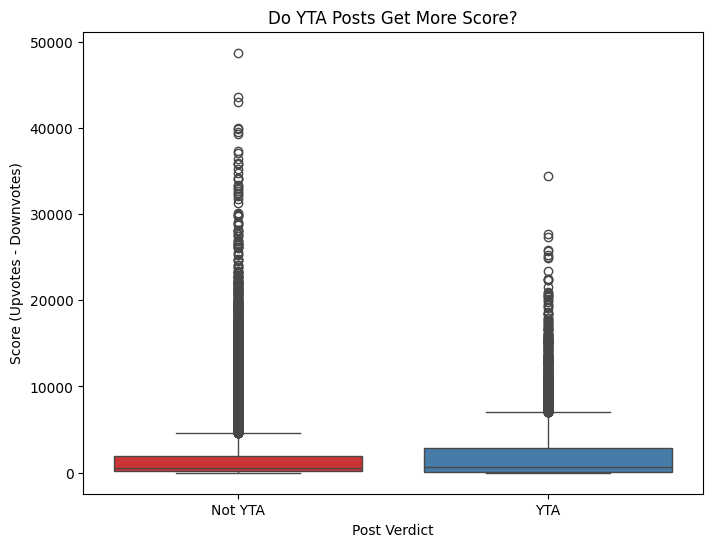
\includegraphics[width=1\linewidth]{resources/score-vs-verdict.png}
    \caption{Puntuación contra el veredicto}
    \label{fig:score-verdict}
\end{figure}

Finalmente, la figura \ref{fig:common-words} muestra algunas de las palabras más utilizadas son palabras muy comunes en la descripción de una historia. La palabra más utilizada es 'said', seguida de 'told' y 'just'. Esto es congruente dado que son verbos o formas de entrelazar una historia. Sin embargo,muchas veces tienen significados semánticos interesantes, donde se habla mucho de las otras personas de una familia "sister", "mom", "family", "wife", etc. Es interesante denotar que en su mayoría son palabras para referirse a personas del género femenino.

\begin{figure}
    \centering
    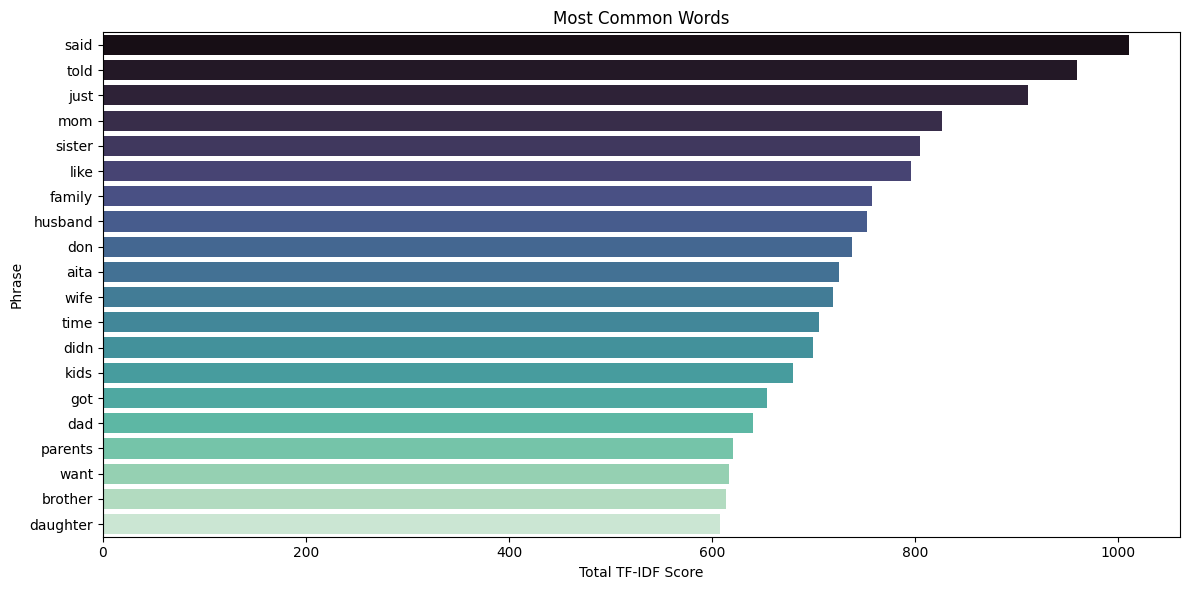
\includegraphics[width=1\linewidth]{resources/common-words.png}
    \hfill
    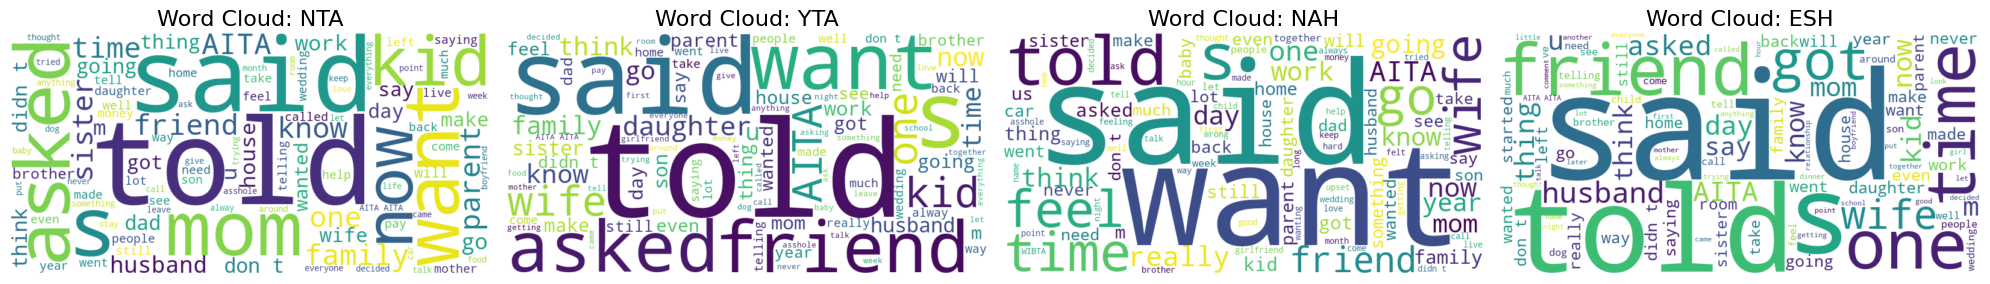
\includegraphics[width=1\linewidth]{resources/word-clouds.png}
    \caption{Palabras más utilizadas, separadas también por clase}
    \label{fig:common-words}
\end{figure}

\subsubsection*{Agrupamiento semántico de temas}

Con el fin de explorar patrones temáticos dentro del corpus, se aplicó un algoritmo de agrupamiento semántico sobre las representaciones vectoriales de las publicaciones, lo cual permitió identificar \textbf{cinco clústeres dominantes}. Cada clúster agrupa publicaciones según vocabulario y contexto compartido, revelando los principales ejes narrativos de los conflictos analizados. Entre los temas más representativos se encuentran: \emph{relaciones de pareja y conflictos matrimoniales}, \emph{dinámicas familiares con hijos}, \emph{disputas con padres y suegros}, \emph{problemas relacionados con mascotas en el hogar}, y \emph{malentendidos en la convivencia}. Esta segmentación temática no solo aporta una visión cualitativa del contenido, sino que también abre la posibilidad de incorporar contexto semántico como variable adicional en futuros modelos de clasificación. Los gráficos \ref{fig:clusters} visualizan los agrupamientos encontrados.


\begin{figure}
    \centering
    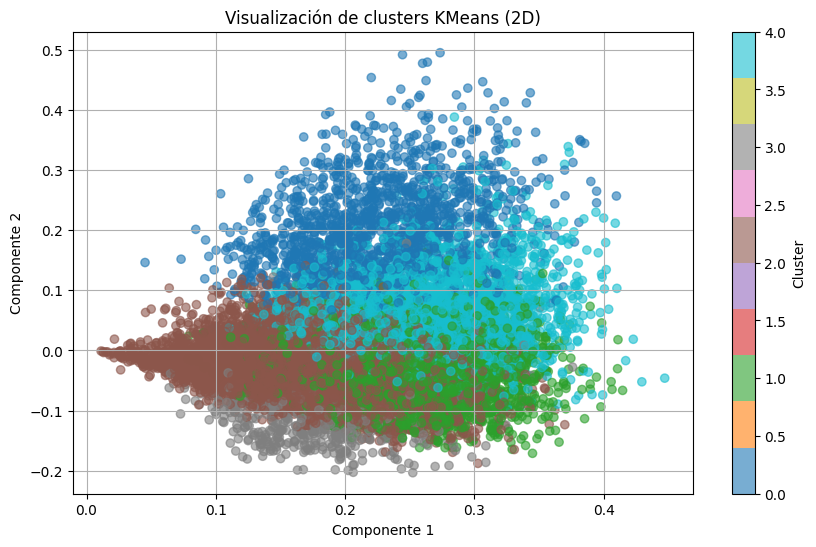
\includegraphics[width=0.45\textwidth]{resources/clusters.png}
    \hfill
    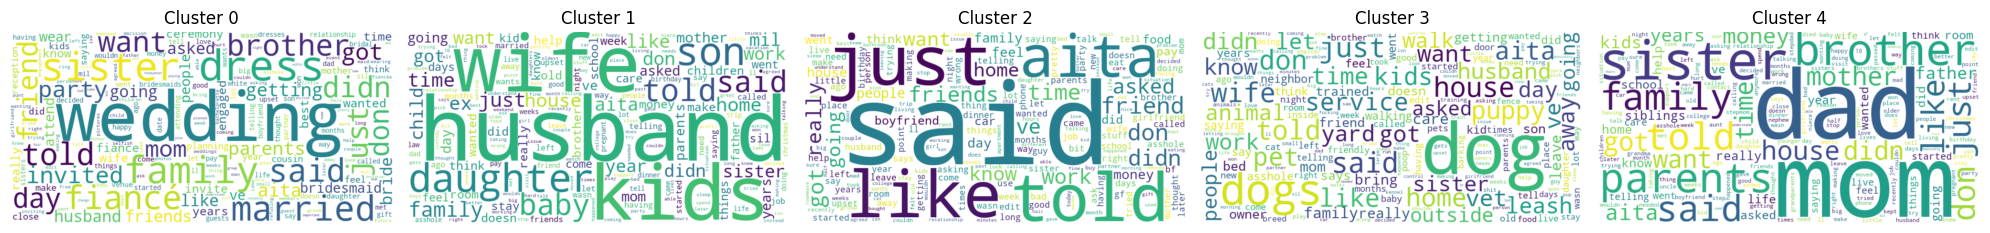
\includegraphics[width=0.45\textwidth]{resources/clusters-2.png}
    \caption{Gráfico de agrupamientos encontradas sobre los datos}
    \label{fig:clusters}
\end{figure}


\subsubsection*{Análisis de sentimiento}

Con el fin de encontrar otros patrones no inherentes a los datos, sino que son observables a través de los mismos, se realizó un análisis de sentimientos (con un modelo pre-entrenado) con el fin de entender si el sentimiento es positivo o negativo dependiendo de la clase. En la figura \ref{fig:sentiment-analysis} se puede ver que en su gran mayoría, los sentimientos que encuentra el modelo son negativos. Lo que tiene mucho sentido. Los usuarios que publican en esta comunidad lo hacen con un propósito de desahogarse, de poder sentir apoyo de otras personas y tener una visión externa de la situación en la que se encuentran.

\begin{figure}
    \centering
    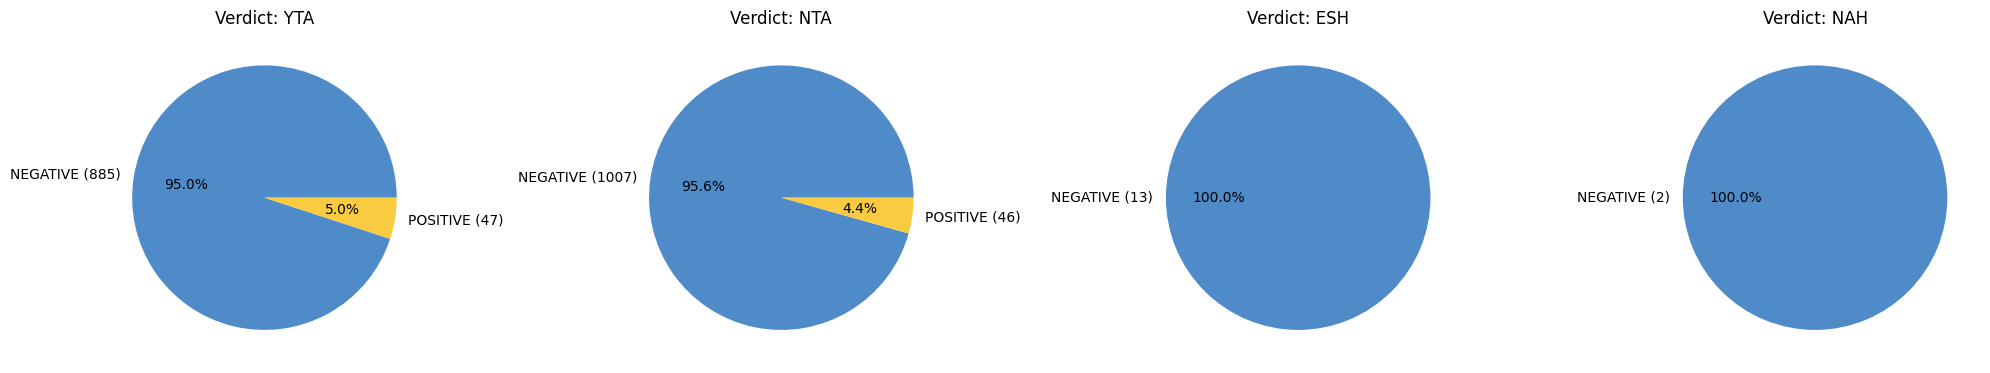
\includegraphics[width=1\linewidth]{resources/sentiment-analysis.png}
    \caption{Gráfico del análisis de sentimiento realizado}
    \label{fig:sentiment-analysis}
\end{figure}

\subsection{Entrenamiento de modelos}

Finalmente dentro de la metodología tenemos el entrenamiento de modelos. Dentro de los objetivos planteados del proyecto estaba la utilización de diferentes modelos de aprendizaje que combinaran diferentes técnicas; tales como el aprendizaje automático clásico, con modelos como la regresión logística, las máquinas de vectores de soporte, entre otros. Y modelos más avanzados, como los grandes modelos de lenguaje (LLMs), o redes recurrentes.

En este orden de ideas, se escogió trabajar los siguientes modelos: 
\begin{itemize}
    \item Clásicos: Regresión logística, Naive Bayes, Máquinas de vectores de soporte.

    Sobre estos modelos se aplicará el aprendizaje tradicional, donde se vectorizan las entradas, generalmente con un vectorizador \verb|Tf-idf|, con el fin de tener un marco de referencia y encontrar patrones interesantes.
    
    \item Aprendizaje profundo: GRU y BERT (y otras variaciones como RoBERTa, XLM-RoBERTa, entre otros).

    Sobre estos modelos se aplicarán dos técnicas. La primera es el aprendizaje desde cero, con el modelo pequeño de GRU, y la segunda es utilizando aprendizaje por transferencia con modelos de la familia BERT. De estos modelos ya se espera un resultado mucho más confiable considerando su naturaleza no-lineal.
    
    \item Grandes modelos de lenguaje: GPT-4o, Llama 3.1.

    Sobre estos modelos no se hará ninguna clase de entrenamiento o fine-tuning. Esto es porque son demasiado grandes. Sin embargo, como son generativos, tienen la capacidad de generar un razonamiento o pensamiento adicional, por lo cual es interesante utilizarlos y ver (con métricas) qué tanto se comparan con respecto a los otros modelos, considerablemente más simples.
    
\end{itemize}

\subsection{Despliegue}

Para el despliegue, el cual será local y no estará disponible en internet, se desarrollará un backend, que tiene la lógica completa de la aplicación, y trabajará con los modelos finales para retornar las predicciones. El frontend, que estará de cara al usuario final, muestra estos resultados permitiendo al usuario ingresar cualquier input, y entender el comportamiento de los modelos a simple vista.
